\documentclass[11pt]{beamer}
\usetheme{Copenhagen}
\usepackage[utf8]{inputenc}
\usepackage[german]{babel}
\usepackage[T1]{fontenc}
\usepackage{amsmath}
\usepackage{amsfonts}
\usepackage{amssymb}
\usepackage{graphicx}
\author{Steffen Holzer und Ellen Wagner}
\title{Parken vor einem Einkaufszentrum}
%\setbeamercovered{transparent} 
%\setbeamertemplate{navigation symbols}{} 
%\logo{} 
%\institute{} 
\date{\today} 
%\subject{} 
\begin{document}

\begin{frame}
\titlepage
\end{frame}

\begin{frame}
\tableofcontents
\end{frame}


\section{Das allgemeine Parkplatzproblem}
\begin{frame}{Das allgemeine Parkplatzproblem}

Gegeben sei eine (unendlich lange) Einbahnstraße mit Parkplätzen und einem Ziel.
\begin{itemize}
	\item Die Parkplätze können belegt oder leer sein
	\item Ein Auto fährt die Straße entlang und versucht einen Parkplatz nahe des Ziels zu bekommen
	\item Ob ein Parkplatz leer ist oder nicht, sieht das Auto erst wenn es ihn erreicht hat
\end{itemize}
\end{frame}


\section{Das Parkplatzproblem von Hutchinson et al.}
\subsection{Modell}

\begin{frame}{Das Problem von Hutchinson et al.}{Modell}
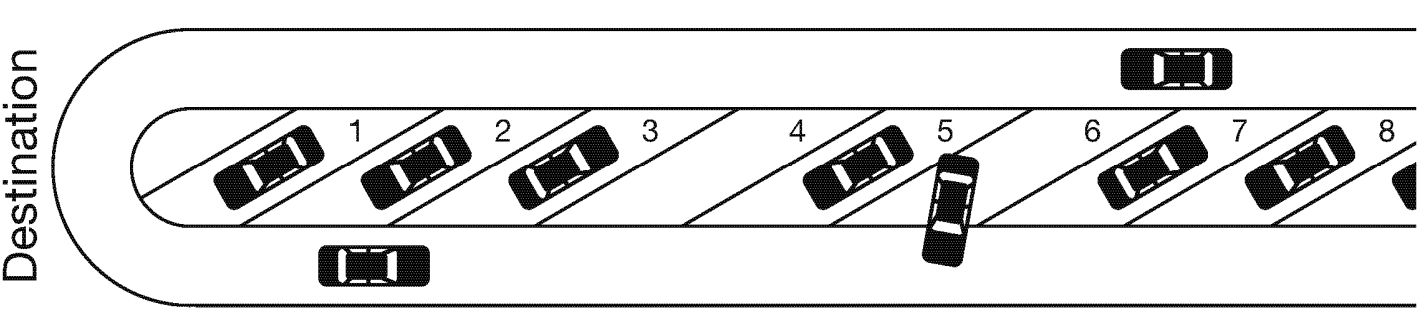
\includegraphics[width=\textwidth]{carparking.png}
\begin{itemize}
	\item Hutchinson, Fanselow, Todd: Car parking as a Game Between Simple Heuristics, 2012
	\item Gebogene Straße mit beidseitig offenen Parkplätzen
	\item Gemeinsames Ziel für alle Autos
\end{itemize}

\end{frame}


\subsection{Annahmen und deren Plausibilität}
\begin{frame}{Das Problem von Hutchinson et al.}{Modellanahmen}
\begin{enumerate}
	\item Diskrete Zeitschritte.
	\begin{itemize}
		\item $\Delta t = 1 \Leftrightarrow $Auto bewegt sich zum nächsten Parkplatz
	\end{itemize}
	\item Autos wählen vor Simulationsbeginn gleichverteilt einen eindeutigen Zeitpunkt, zu dem sie die Straße betreten
	\item Ein Auto ,,sieht'' den Parkplatz an dem es aktuell ist sowie dessen Nachfolger
	\pause
	\begin{itemize}
		\item Würde das Auto den Parkplatz $n$ nehmen aber $n-1$ ist frei wird $n$ abgelehnt
		\item Wird ein Parkplatz $n$ gewählt, parkt das Auto für $\Gamma (X)+10\cdot n$ Zeitschritte
		\item Mittelwert von $\Gamma$ ist 30 min mit einem Maximum von 3h
	\end{itemize}
\end{enumerate}
\end{frame}

\begin{frame}{Das Problem von Hutchinson et al.}{Modellanahmen}
	\begin{enumerate}
		\setcounter{enumi}{3}
		\item Verteilung der Autos
		\begin{itemize}
			\item Eine Zeiteinheit sind $0.75s$
			\item Ein Simulationstag hat 9h
			\item Insg. 1080 Autos $\Rightarrow 2 \frac{Auto}{min}$
		\end{itemize}
		\item Die Verteilung der Autos ist gleichförmig
		\item Autos drehen am Ziel ohne Zeitverlust
	\end{enumerate}
\end{frame}

\subsection{Heuristik}

\begin{frame}{Das Problem von Hutchinson et al.}{Verwendete Heuristik}
Hier: Beschränkung auf ,,Fixed-Distance''-Heuristik, die einen freien Parplatz wählt, wenn
	\begin{itemize}
		\item dieser höchstens noch $n$ Schritte vom Ziel entfernt ist, oder
		\item man den Scheitelpunkt passiert hat
	\end{itemize}
\end{frame}

\begin{frame}{Das Problem von Hutchinson et al.}{Evolutionäre Heuristik}
\begin{itemize}
	\item Simulation geht über 10.000 Tage
	\item Tag 1: Jedes Auto startet mit zufälligem Heuristikparameter $n\in \lbrack 0,150 \rbrack$
	\item Nach jedem Tag:
	\pause
	\begin{itemize}
		\item Die besten $10\%$ der Parameter werden von $90\%$ der Autos übernommen
		\begin{itemize}
			\item Parametergüte bezieht sich auf Reisezeit $t_r = t_{suche}+10\cdot d + (150-d)$, $d$ Entfernung zum Ziel
		\end{itemize}
		\item Restliche $10\%$ wählen wieder zufällige Parameter
	\end{itemize}
	\item[$\Rightarrow$] Nash-Equilibrium
\end{itemize}
\end{frame}

\subsection{Ergebnis}

\begin{frame}{Das Problem von Hutchinson et al.}{Ergebnis}
	\begin{itemize}
		\item Equilibrium stellt sich ein für $n=31$
		\item $\varnothing t_r = 478s = 637 ticks$
		\item $\varnothing d = 34,6$
	\end{itemize}
\end{frame}

\section{Unsere Simulation}

\subsection{Frage}

\begin{frame}{Fragestellung}
Bleibt dieser Parameter stabil unter sich ändernder Frequenz ankommender Autos?
\end{frame}

\subsection{Unterschiede im Modell}

\begin{frame}{Unsere Simulation}{Unterschiede zu Hutchinson et al}
\begin{itemize}
	\item Ein 12h (57600 Ticks) Tag mit 3 Ankunftsverteilungen 
	\item Wartezeit zwischen den Autos zufällig und gleichverteilt
	\item Heuristik lernt während des Tages
	\item Durchqueren des Scheitelpunkts dauert einen Tick
\end{itemize}
\end{frame}



\subsection{Simulations-Parameter}

\begin{frame}{Unsere Simulation}{Parameter}
\begin{itemize}
	\item 3 Phasen Gleichverteilung
	\begin{itemize}
		\item Jeweils 4h
		\item Mittlere Ankunftszeiten von 2,1 und 4 Autos pro Minute
	\end{itemize}
	\item Warteverteilung:  $\Gamma$-Verteilung mit Mittelwert $30min$ und Maximum von $1h$
	\item potentiell unendlich viele Autos
\end{itemize}
\end{frame}

\subsection{Lernende Heuristic}

\begin{frame}{Unsere Simulation}{Modifizierte Annahmen}

	\begin{itemize}
		\item Merkt sich die letzten 30 Parameter, die einen Parkplatz gefunden haben
		\item Die ersten 30 Parameter sind zufällig gleichverteilt in $\lbrack 0,150\rbrack$
		\item Neue Heuristiken werden mit dem gelernten Wert initialisiert:
		\begin{itemize}
			\item Wähle die 10 Parameter, die am Nächsten zum Ziel geparkt haben
			\item Initialisiere die neue Heuristik mit dem gewichteten Mittel der 10 ($n_e=\frac{\sum a_i\cdot n_i}{\sum a_i}$)
			\item wobei $a_i = \Biggl\lbrace 
				\begin{matrix}
					10 & \text{ Parkplatz im vorderen Viertel}\\
					3 & \text { Parkplatz liegt im 2. vorderen Viertel}\\
					0 & \text{ sonst}
				\end{matrix}$
			\item $15\%$ der Heuristiken werden zufällig initialisiert
		\end{itemize}
	\end{itemize}

\end{frame}


\subsection{Ergebnisse}

\begin{frame}{Unsere Simulation}{Ergebnisse --  Parameterverlauf}
	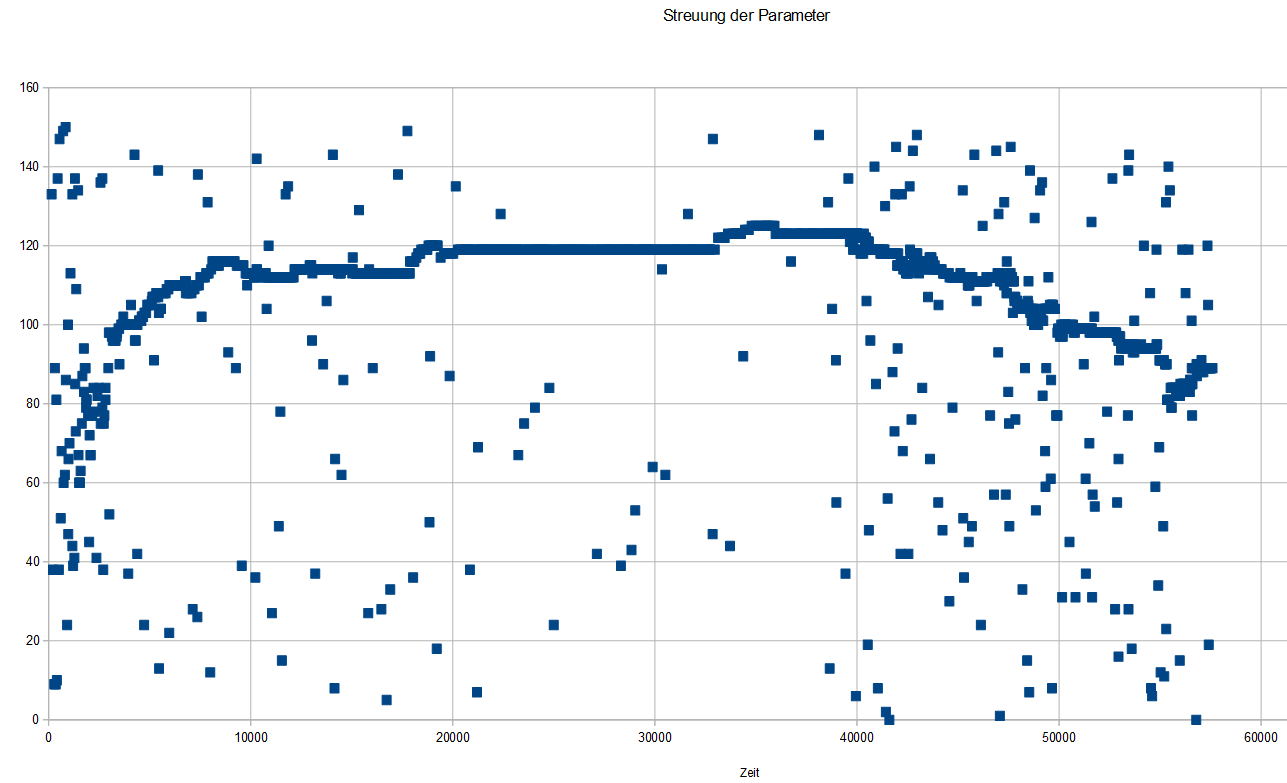
\includegraphics[width=\textwidth]{streuung.png}
\end{frame}

\begin{frame}{Unsere Simulation}{Ergebnisse -- Abstand und Häufigkeit bei $2\frac{Autos}{min}$}
	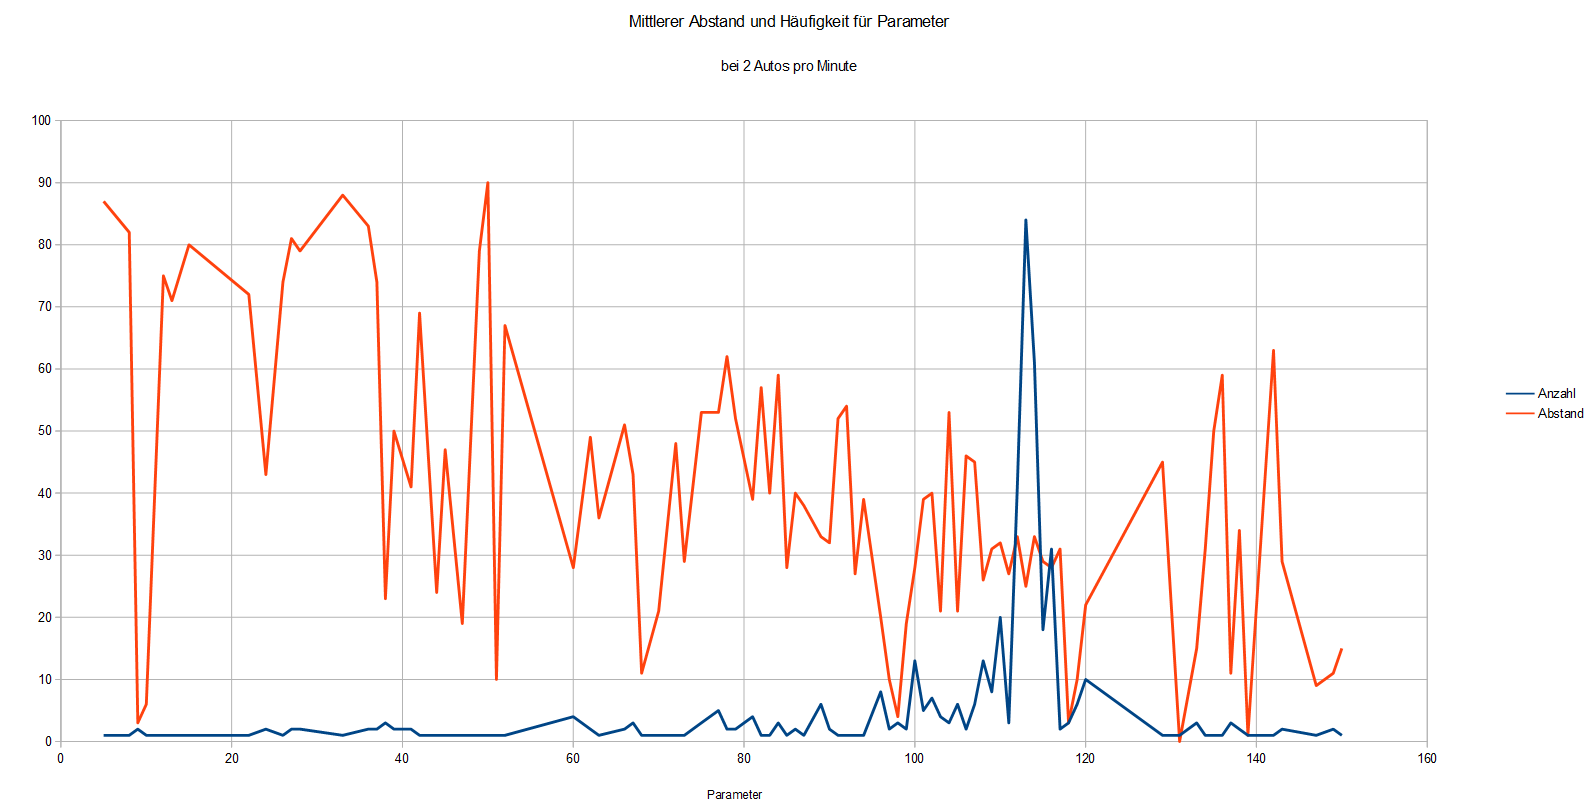
\includegraphics[width=\textwidth]{ma_1.PNG}
\end{frame}

\begin{frame}{Unsere Simulation}{Ergebnisse -- Abstand und Häufigkeit bei $1\frac{Autos}{min}$}
	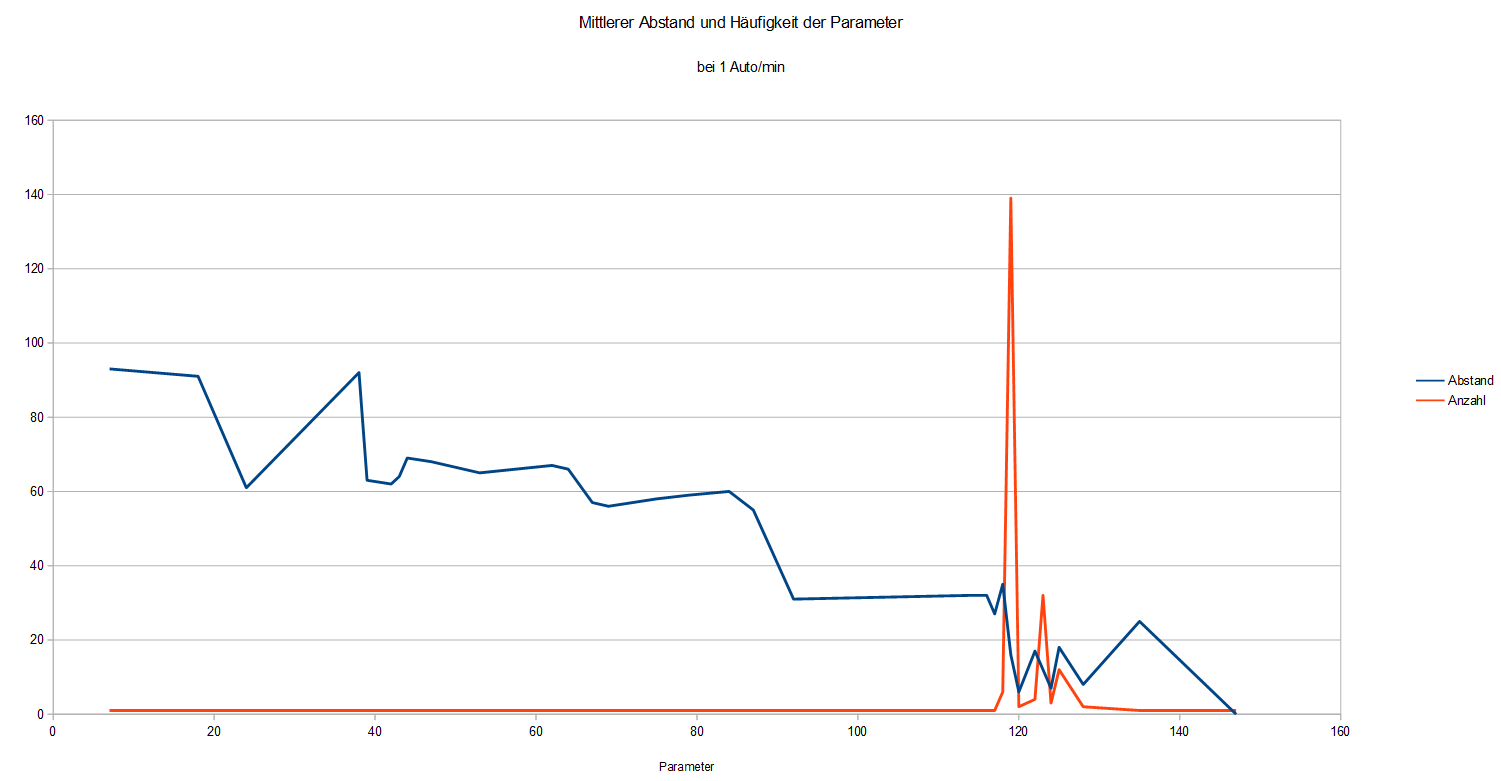
\includegraphics[width=\textwidth]{ma_2.PNG}
\end{frame}

\begin{frame}{Unsere Simulation}{Ergebnisse -- Abstand und Häufigkeit bei $4\frac{Autos}{min}$}
	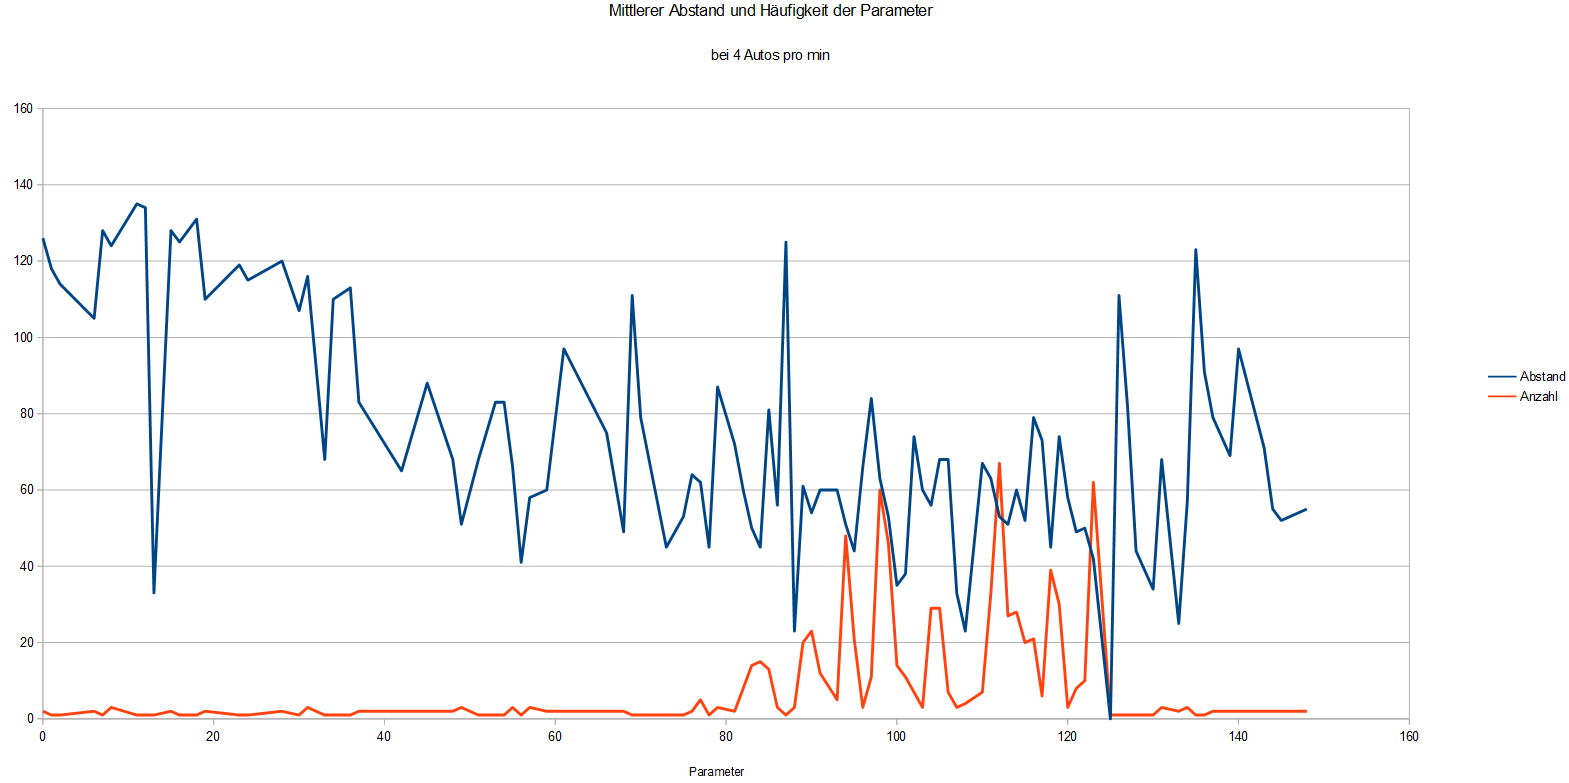
\includegraphics[width=\textwidth]{ma_3.PNG}
\end{frame}

\begin{frame}{Unsere Simulation}{Ergebnisse}
\begin{itemize}
	\item Bei $2 \frac{Autos}{min}$ wird ein ähnlicher Wert wie bei Hutchinson et al. angenommen
	\item Der Parameterwert steigt für geringe und fällt für hohe Frequenzen
\end{itemize}
\end{frame}

\begin{frame}{Unsere Simulation}{Ergebnisse -- Parameterverlauf bei langer hoher Frequenz}
	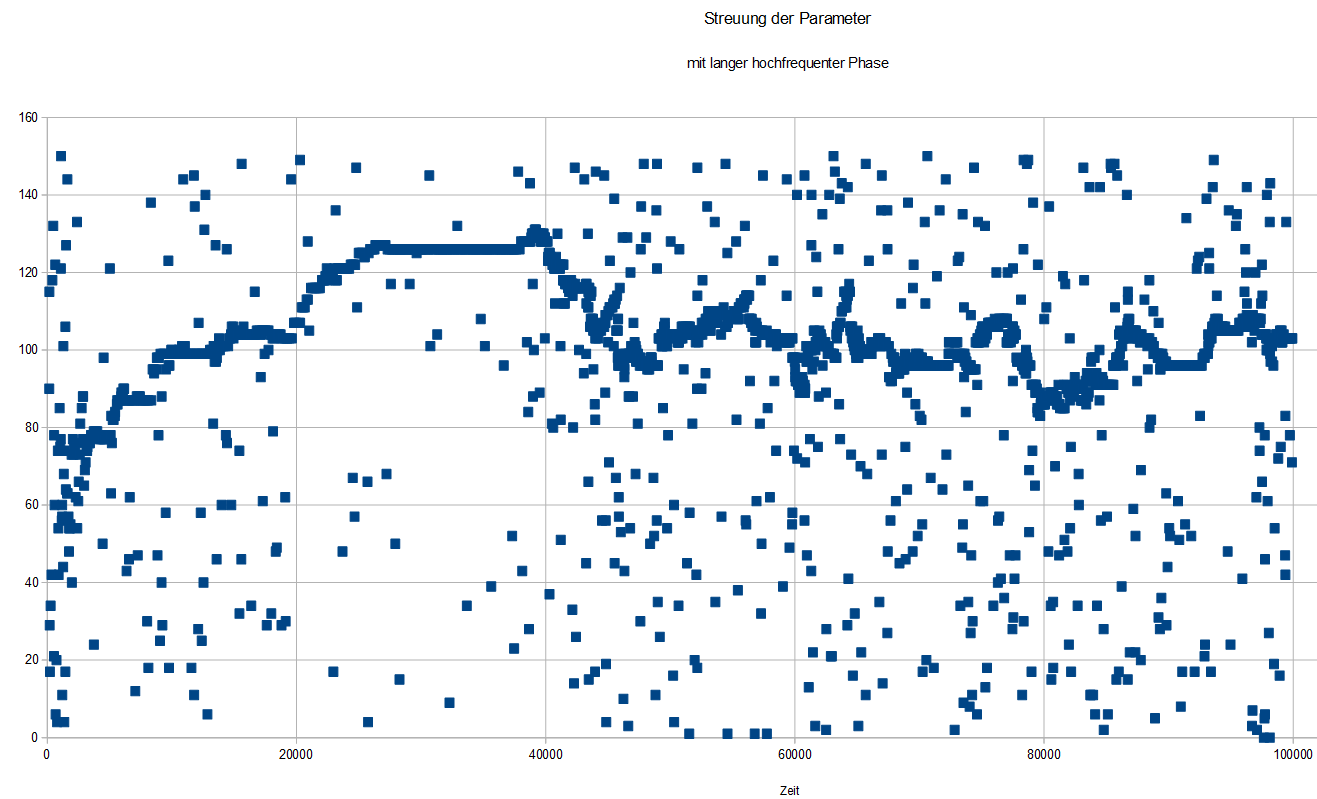
\includegraphics[width=\textwidth]{streuung_long.PNG}
\end{frame}

\section{Ausblick}

\begin{frame}{Ausblick}
	\begin{itemize}
		\item Untersuchung weiterer Heuristiken
		\item Untersuchung der Belegungswahrscheinlichkeit von Parkplätzen
		\item Direkter Wettkampf der Heuristiken unter verschiedenen oder wechselnden Frequenzen
	\end{itemize}
\end{frame}

\section{Schuleinsatz}

\begin{frame}{Schuleinsatz}
\begin{itemize}
	\item Programmieren der Simulation nicht trivial, Verbindung zum Informatikunterricht
	\item Austesten von Heuristiken aber auch enaktiv möglich
	\item Auswertung auch ohne Simulation in GeoGebra (oder Calc) möglich 
\end{itemize}
\end{frame}

\begin{frame}
\begin{center}
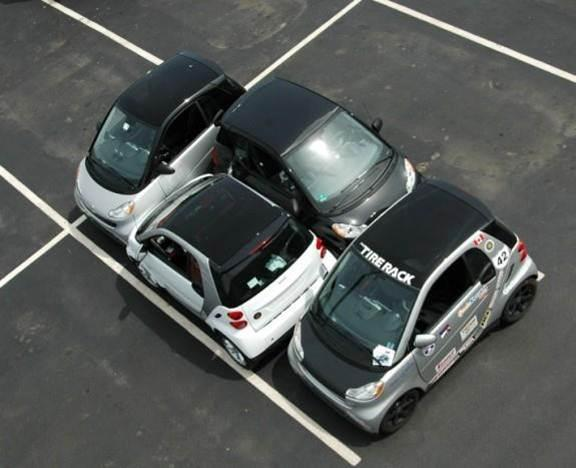
\includegraphics[scale = 0.25]{quer_parken_1.jpg}\\
Danke für Eure Aufmerksamkeit!
\end{center}
\end{frame}


\end{document}